\iffalse
\documentclass[journal,12pt,twocolumn]{IEEEtran}
\usepackage{amsmath,amssymb,amsfonts,amsthm}
\usepackage{txfonts}
\usepackage{tkz-euclide}
\usepackage{listings}
\usepackage{gvv}
\usepackage[latin1]{inputenc}
\usepackage{adjustbox}
\usepackage{array}
\usepackage{tabularx}
\usepackage{pgf}
\usepackage{lmodern}
\usepackage{circuitikz}
\usepackage{tikz}
\usepackage{graphicx}
\begin{document}
\bibliographystyle{IEEEtran}

\vspace{3cm}

\title{}
\author{EE23BTECH11047 - Deepakreddy P
}
\maketitle
\newpage
\bigskip

\noindent \textbf{44} \quad The switch $S_1$ was closed and $S_2$ was open for a long time. At t=0,switch $S_1$ is opened and $S_2$ is closed,simultaneously. The value of $i_c(0^{+})$, in amperes, is  \hfill (GATE EC 44)

\begin{figure}[ht]
  \centering
  \begin{adjustbox}{width=\columnwidth}
      \begin{circuitikz}[american]
   \draw (0,0) to [isource, l=1A] (0,4) ;
   \draw (0,0) to [short] (3,0) to [C = 0.01F] (3,4) to [short] (6,4) to [R = 100 $\Omega$] (6,2) to [L = 1H] (6,0) to [short] (9,0) to [R = 25 $\Omega$] (9,4) to [short] (6,4) ;
   \draw (3,0) to [short] (6,0) ;
   \draw (0,4) to [ospst = $S_1$] ++(3,0); 
   \draw (7.5,4) to [cspst = $S_2$] ++(0,-2);
   \draw (7.5,2) to [short] (6,2) ;
   \draw (3,4) to [short ,i = $i_c$] (3,3);
   
\end{circuitikz}

  \end{adjustbox}
  \caption{Circuit 1}
\end{figure}

\solution
\fi
\\
1) Switch $S_1$ was closed and $S_2$ was open 
\begin{figure}[ht]
  \centering

      \begin{circuitikz}[american]
   \draw (0,0) to [isource, l=1A] (0,4) ;
   \draw (0,0) to [short] (3,0);
   \draw (0,4) to [short] (9,4) to [R=25$\Omega$] (9,0) to [short] (3,0);
   \draw (6,4) to [R = 100$\Omega$] (6,0);
   \draw (3,4) -- ++(0,-1.5)
   to [open, v = $V_c(0^{-})$, o-o] ++(0,-1.5) -- ++(0,-1);
   \draw (6,1) to [short ,i = $i_L \brak{0^-}$] (6,0);
   
\end{circuitikz}


  \caption{$S_1$ is closed and $S_2$ is open}
\end{figure}

\begin{align}
    R_{eff} &= \frac{25\brak{100}}{\brak{25+100}} \Omega \\
    R_{eff} &= 20 \Omega 
\end{align}
\begin{align}
    V_c \brak{0^-} &= 1 \brak{R_{eff}}\\
    V_c \brak{0^-} &= 20V
\end{align}

\bigskip

2) Switch $S_1$ is open and $S_2$ was closed\\

\bigskip

At $t=0^{+}$ The capacitor is charged. Thus, it acts as a voltage source.The inductor acts as the current source.

\bigskip

\begin{figure}[ht]
  \centering
      \begin{circuitikz}[american]
   \draw (3,4) to [C=$\frac{1}{sC} $ ](3,2) to [V=$\frac{V_c \brak{0^-}}{s}$ ] (3,0) ;
   \draw (3,4) to [short] (9,4);
   \draw (8,0) to [V=$L i_L \brak{0^-}$] (8,2) ;
   \draw (8,4) to [L = $Ls$](8,2) ;
   \draw (8,4) to [short] (10,4) to [R = 25 $\Omega$] (10,0) to [short] (8,0);
   \draw (3,0) to [short] (8,0) ;
   \draw (3,2) to [short, i = $i_{c} \brak{s}$] (3,1.5);
   \draw (10,1) to [short ] (10,0);
\end{circuitikz}

  \caption{$S_1$ is open and $S_2$ is closed}
\end{figure}

\bigskip

By Superposition Theorem\\
\bigskip
Case (i):
\begin{figure}[ht]
  \centering

      \begin{circuitikz}[american]
   \draw (3,4) to [C=$\frac{1}{sC} $ ](3,2) to [V=$\frac{V_c \brak{0^-}}{s}$ ] (3,0) ;
   \draw (3,4) to [short] (9,4);
   \draw (8,4) to [L = $Ls$](8,0) ;
   \draw (8,4) to [short] (10,4) to [R = 25 $\Omega$] (10,0) to [short] (8,0);
   \draw (3,0) to [short] (8,0) ;
   \draw (3,2) to [short, i = $i_{c}^1 \brak{s}$] (3,1.5);
   \draw (10,1) to [short] (10,0);
\end{circuitikz}


  \caption{Circuit 4}
\end{figure}

\begin{align}
     \brak{\frac{25\brak{Ls}}{25 + Ls} + \frac{1}{sC}}i_{c}^1 \brak{s} + \frac{V_c \brak{0^-}}{s} = 0\\
     i_{c}^1\brak{s} =  -\frac{V_c\brak{0^-}}{s} \brak{\frac{25sC+LCs^2}{25LCs^2 +Ls + 25}}\\
     i_{c}^1\brak{s} =  -\brak{\frac{5+0.2 s}{0.25s^2 +s + 25}} \label{eq:eq.EC.44.1}
\end{align}

\newpage
Case (ii):

\begin{figure}[ht]
  \centering

      \begin{circuitikz}[american]
   \draw (3,4) to [C=$\frac{1}{sC} $ ] (3,0) ;
   \draw (3,4) to [short] (9,4);
   \draw (8,0) to [V=$L i_L \brak{0^-}$] (8,2) ;
   \draw (8,4) to [L = $Ls$](8,2) ;
   \draw (8,4) to [short] (10,4) to [R = 25 $\Omega$] (10,0) to [short] (8,0);
   \draw (3,0) to [short] (8,0) ;
   \draw (3,3) to [short, i = $i_{c}^2 \brak{s}$] (3,2.5);
   \draw (10,1) to [short] (10,0);
\end{circuitikz}


  \caption{Circuit 5}
\end{figure}

\begin{align}
    Li_L \brak{0^-} + \brak{\frac{25}{25sC + 1} + Ls} i_{c}^2 \brak{s} = 0
\end{align}
\begin{align}
     0.2 &= - \brak{\frac{25LCs^2 + Ls + 25}{25sC + 1}} i_{c}^2 \brak{s}\\
    i_{c}^2 \brak{s} &= -\brak{\frac{0.05s + 0.2}{0.25s^2 + s + 25}}  \label{eq:eq.EC.44.2}
\end{align}

From eq \eqref{eq:eq.EC.44.1} and eq \eqref{eq:eq.EC.44.2}

\begin{align}
     i_c \brak{s} &= i_{c}^1 \brak{s} + i_{c}^2 \brak{s}\\
     i_c \brak{s} &= - \brak{\frac{0.25s +5.2}{0.25s^2 + s + 25}} \label{eq:eq.EC.44.3}
\end{align}

Using Inverse Laplace Transform 

From eq \eqref{eq:eq.EC.44.3}

\begin{align}
    i_{c} \brak{t} &= - e^{-2t} \brak{\cos\brak{4\sqrt{6}\, t} + \frac{18.8}{4\sqrt{6}}\sin{\brak{4\sqrt{6}\, t}}}\\
    i_{c} \brak{0^+} &=-1A 
\end{align}

\begin{figure}[ht]
   \centering
   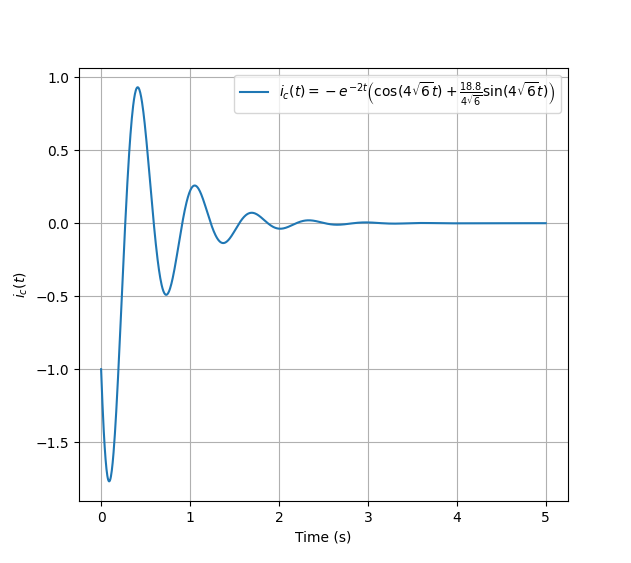
\includegraphics[width=1.2\columnwidth]{2023/EC/44/figs/abd.png}
   \caption{Plot of $i_c \brak{t}$ vs time}
\end{figure}


\begin{table}[ht]

       \setlength{\arrayrulewidth}{0.3mm}
\setlength{\tabcolsep}{20pt}
\renewcommand{\arraystretch}{1.3}



\begin{tabular}{|c|c|c|}
\hline

Parameter& Description & Remarks\\
\hline
$V_c\brak{0^{-}}$ & Voltage across capacitor when t$<$0 & 20V\\
\hline
$i_L \brak{0^-}$ & current across inductor when t$<$0 & $0.2 $  \\
\hline
$i_L \brak{0^+}$ & current across inductor when t$>$0 & $0.2 $\\
\hline
$C$ & Capacitance & 0.01F\\
\hline
$L$ & Inductance & 1H\\
\hline

\end{tabular}



    \caption{Parameters}
    \label{tab:Gate.ec.44.1}

\end{table}

\begin{figure}[ht]
   \centering
   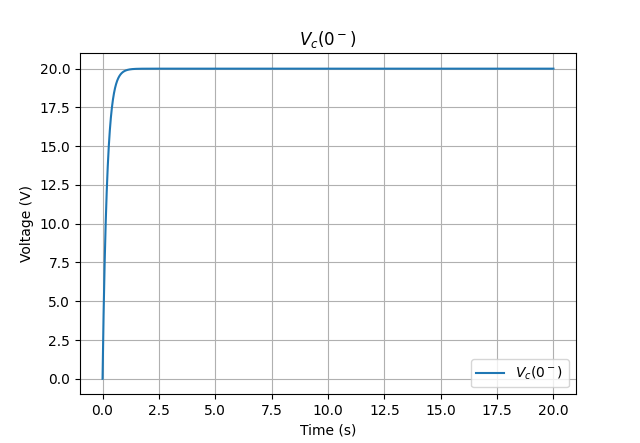
\includegraphics[width=1.2\columnwidth]{2023/EC/44/figs/ckt2.png}
   \caption{Plot of $V_c(0^-)$ vs time}
\end{figure}

%\end{document}



